 %%%%%%%%%%%%%%%%%%%%%%%%%%%%%%%%%%%
% Learning Processes
%%%%%%%%%%%%%%%%%%%%%%%%%%%%%%%%%%%
\section{Learning Processes}
Seeing as how math is causing such difficulties for students, it is relevant to look at how math is being taught and how students are being taught in general. In this chapter three different teaching styles will be presented, along with a section about how tasks are important for learning. At the end there will be a discussion about virtual learning tools and their impact.

%%%%%%%%%%%%%%%%%%%%%%%%%%%
% Teaching styles
%%%%%%%%%%%%%%%%%%%%%%%%%%%
\subsection{Teaching styles}
When teaching adolescents, identity development is very important. Therefore teaching styles which can help identity development will help to engage students in the education. There are several different teaching styles and practices, which describe how a teacher can help his students achieve the best learning. In this paper three teaching styles, described and researched by Kristy S. Cooper\cite{CooperElicitingPractices} will be discussed, as they have all been tested and discussed in length by Cooper and they all seem to be generally applicable:

\begin{itemize}
\item \textbf{Connective Instruction} is a teaching practice where the teacher focuses on helping the students make personal connections to a class. It consists of six different means to engage the students and help them learn: promoting relevance, conveying care, demonstrating understanding of students, providing affirmation, relating to students through humor and enabling self-expression. Each of these individually have been proven to help a teacher to get through to the students.
\item \textbf{Academic Rigor} focuses on the academic part of learning, mainly through focusing on three points: providing challenging work, pushing students through academic press and conveying passion for content. Academic rigor emphasizes hard work and academic success, reinforcing the academic focus of the class.
\item \textbf{Lively Teaching} focuses on emphasizing active delivery of instruction. It is made up of three practices: Using games and fun activities, having students work in groups and assigning projects. This method of teaching utilizes the fact that students actively participate in what is happening, and are working together.
\end{itemize}

\noindent
Lively teaching is focused on teaching a class collectively and less on the individual student, whereas the academic rigor and connective instruction are more easily applied to helping the individual student. Neither of them are mutually exclusive however and a combination of the different teaching styles is concluded by Cooper to generally be the most beneficial for giving the students the best learning experience.
\newline\newline
The research of the teaching styles by Cooper has only been carried out in America, but in this report it is assumed that the theory of these teaching styles is widely applicable and functioning at least in the rest of the western world. Looking at how these teaching styles fit into the danish education system, two of the key principles for education in Denmark, according to the Danish ministry of Higher Education and Science are active participation and project work \cite{MinistryofHigherEducationandScience2018PrinciplesForskningsministeriet}. Active participation is covered by all three of these teaching styles, as they all in some way focus on motivating the students to participate in the education. Connective instruction attempts to encourage the active participation by having the students relate to the rest of the class and the teacher, the academic rigor by motivating the students academically and lively teaching by focusing on different activities. Project work is specifically mentioned in the definition of the lively teaching style, and as such this also fits into the danish educational principles.
\newline\newline
Another way it is made clear how the teaching styles fit into the danish way of educating students is when looking at \newacr{Problem Based Learning}{PBL}. PBL is a way to have students learn, through focusing on a specific problem and how to solve it, especially used during project work. PBL is used both in a lot of the Danish Gymnasiums and in some Danish universities. Looking at some of the principles behind PBL \cite{Holgaard2014PBL-ProblembaseretUddannelser}, it is clear that they line up with the teaching styles presented by Cooper. In PBL there is a clear focus on the relevance of whatever subject is being worked on, and how the knowledge can be practically applied. Just like the part of connective instruction is promoting the relevance of the subject. An important part of PBL is also the group-based work, where the teacher only functions as a supervisor or guide, instead of having the teacher decide everything. This fits well with connective instruction where you enable self expression, and lively teaching, which focuses on group and project-based work. It also fits with academic rigor, seeing as how the point of using PBL and how much it relates to the real world, shows the importance of what the students are being learned, inspiring them to come up with real world solutions. 
\newline\newline
Moreover, according to a paper from Jens Rasmussen \cite{Rasmussen2013CompetenceHotel} the school systems in America and the EU and thereby also Denmark are all similar in that they use what is called a outcome-driven curricula, that means there is a focus on what the students are supposed to achieve with with what they are learning in terms of knowledge, skills and competences. Rasmussen also mentions how the EU has become more similar to America in terms of the focus on education and the way curricula are shaped. In some ways the EU has molded its education policy after America. Since the goals of the education and the way the countries wish to achieve them are similar it can be assumed that since these learning styles work in America they should also be applicable in the EU \cite{Rasmussen2013CompetenceHotel}. 

%%%%%%%%%%%%%%%%%%%%%%%%%%%
% Using tasks in teaching
%%%%%%%%%%%%%%%%%%%%%%%%%%%
\subsection{Using tasks in teaching}
The tasks students are given, and what they learn from them is a key aspect of teaching and learning maths. The tasks should provide a challenge of a fitting difficulty, and the students should have a meaningful reason to engage in the tasks \cite{Clarke2009Tasks123}.
\newline\indent
A teacher should have a professional identity made up of 5 key points: professional language, a personal view on and beliefs about knowledge and learning, knowledge about classroom management, methods and material and competence to judge and diagnose pupils learning in maths and knowledge in maths related to teaching \cite{Clarke2009Tasks123}.

%%%%%%%%%%%%%%%%%%%%%%%%%%%
% Using online and virtual tools
%%%%%%%%%%%%%%%%%%%%%%%%%%%
\subsection{Using online and virtual tools}
\label{sub:using_online_and_virtual_tools}
Using online tools to help with learning, is a way students can learn without needing to sit in a classroom and get help from a teacher. For this reason, online course and virtual teaching tools are becoming more popular. One type of online course is \newacr{Massive Open Online Courses}{MOOCS}, which are courses where thousands of people can sign up at once. Even though many of these courses are made in such a way that they could be a substitute for a similar real life course, it is also used as a supplement to real world education or course, by for example gymnasium students. As seen on \figureref{fig:MOOCS} the number of MOOCS available is rising, meaning they will be able to cover more subjects and be available to more people. Also as it can be seen, using this sort of online tool is popular both in and outside EU.

\begin{figure}[H]
\centering
    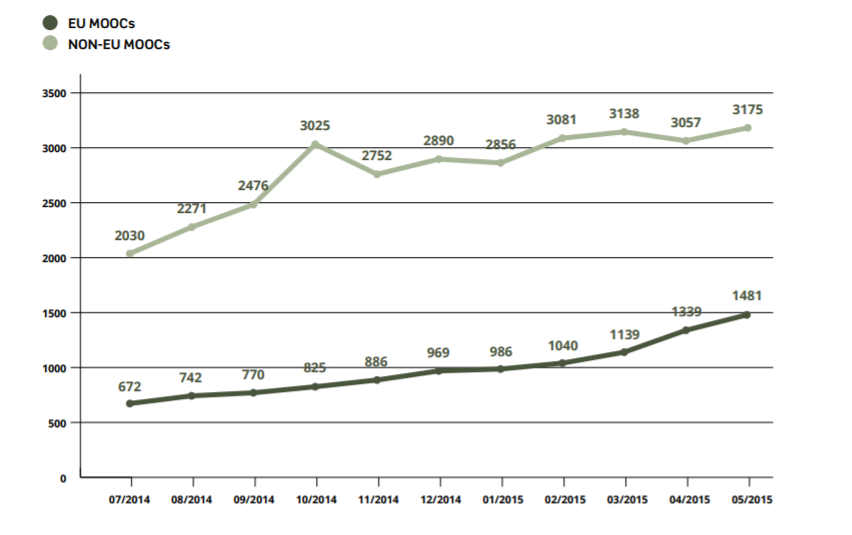
\includegraphics[width=0.75\textwidth]{figures/MOOCS.PNG}
    \caption{Growth in the number of MOOCS available in EU and in NON-EU countries \cite{Warming2016MOOCsPERSPEKTIVER}}
    \label{fig:MOOCS}
\end{figure}

\noindent
Many of these courses are, however, exclusively online which when not taken in concurrence with real-life schooling can cause problems. Attendance and whether or not the students are cheating can, among other things, be hard to monitor in an online course and can cause a low quality in the education of the studies. According to Hani Morgan\cite{Morgan2015ThePupils} studies show that in some circumstances online conditions helped students perform better than students only receiving face-to-face instructions. Morgan also mentions that several studies have also shown that an approach using both traditional face-to-face education combined with online instruction yields the best results. Since many students today already use technology on an everyday basis, using technology for education is also a good way to connect to the students making their everyday lives feel more in line with the education they are receiving. According to Morgan an online teacher must take the following actions to achieve the best results.

\begin{itemize}
\item Experiment with new technologies that may enhance virtual learning environments
\item Include elements in their courses reflecting student interests
\item Take the right steps for students expressing personal crisis
\item Deliver the content in a manner consistent with the learning styles of students
\item Motivate students
\item Continuously improve their technology skills
\item Promote and encourage communications between students
\item Communicate with students in many ways
\item Provide quick feedback
\item Do their best to help students succeed
\end{itemize}